\documentclass[a4paper,12pt]{article}
\usepackage{amsmath,amsfonts,amsthm,amssymb, mathtools,steinmetz, gensymb, siunitx}	% LOADS USEFUL MATH STUFF
\usepackage{xcolor,graphicx}
\usepackage[a4paper]{geometry} 				% ADJUSTS PAGE
\usepackage{setspace}
\usepackage{physics}
\usepackage{caption}
\usepackage{tikz}
\usepackage{pgf,tikz,pgfplots}
\usepackage{mathrsfs}
\usepackage{amsbsy}
\usepackage{fancyhdr}
\usepackage{float}
\usepackage{array}
\usepackage{booktabs}
\usepackage{newpxtext}
\usepackage{unicode-math}
\setmathfont{Libertinus Math}

\usetikzlibrary{decorations.pathreplacing,decorations.markings}
\usepgfplotslibrary{fillbetween}

\newgeometry{left=1cm,top = 2.5cm, bottom = 1.75cm, right = 1cm}

\newcommand{\defeq}{:=}
\newcommand\block[1]{\hspace*{#1}}
\newcommand{\rpm}{\sbox0{$1$}\sbox2{$\scriptstyle\pm$}
	  \raise\dimexpr(\ht0-\ht2)/2\relax\box2 }
\newcommand{\af}{\pmb{\hat a_1}}
\newcommand{\as}{\pmb{\hat a_2}}
\newcommand{\at}{\pmb{\hat a_3}}
\newcommand\uv[1]{\pmb{\hat {#1}}}
\newcommand\vect[1]{\pmb{{#1}}}
\newcommand\dprod{\pmb{\cdot}}
	  
\pgfplotsset{compat=newest}
\newlength{\QNo}
\settowidth{\QNo}{2.}

\newlength{\QLetter}
\settowidth{\QLetter}{(a)}

\pagestyle{fancy}
\rhead{Solid State Physics Problem Set}
\lhead{J. L. Gouws}


\begin{document}
\fontencoding{T1}
\fontfamily{ppl}\selectfont
{\Large \textbf{Solid State Physics Assignment 1}} \hfill {\Large \textbf{J L Gouws}}\\
\block{1.0cm} {\large \textbf{\today}} \hfill {\large \textbf{19G4436}}\\
\thispagestyle{empty}
\fontencoding{T1}

1.
\begin{minipage}[t]{0.9\textwidth}
  a).
  \begin{minipage}[t]{\textwidth}
    For a given plane $[hkl]$, we can see that the plane intersects the basis vectors at \footnotemark:\\
    \begin{equation*}
      \frac{1}{h} \af \qquad \frac{1}{k} \as \qquad \frac{1}{l} \at
    \end{equation*}
    These might not be defined if $h$, $k$, or $l$ is equal to zero, but we will deal with that difficulty later.
    It follows that the vectors:
    \begin{equation*}
      \vect{ u'} = \frac{1}{h} \af - \frac{1}{k} \as \qquad \vect{v'} = \frac{1}{h} \af - \frac{1}{l} \at \qquad  \vect{w'} = \frac{1}{k} \as - \frac{1}{l} \at
    \end{equation*}
    are parallel to the plane, in fact they completely determine the orientation of the plane.
    Since we are only interested in the orientation of the plane, we can multiply each of the vectors by a scalar, which does not change the direction of the vectors.
    We define:
    \begin{equation*}
      \vect{u} \defeq hk \vect{u'} = k \af - h \as \qquad \vect{v} \defeq hk \vect{u'}= l \af - h \at \qquad  \vect{w} \defeq hk \vect{u'} = l \as - k \at
    \end{equation*}
    And we no longer have to worry about infinite vectors.
    Since these vectors span the plane and determine its orientation, we can see if they are perpendicular to $\pmb{G}$
    \begin{gather*}
      \pmb{G} \dprod \pmb{u} = (h \uv{b_1} + k \uv{b_2} + l \uv{b_3})\dprod (k \af - h \as)
                             = 2 \pi hk - 2 \pi kh
                             = 0\\
      \pmb{G} \dprod \pmb{v} = (h \uv{b_1} + k \uv{b_2} + l \uv{b_3})\dprod (l \af - h \at)
                             = 2 \pi hl - 2 \pi lh
                             = 0\\
      \pmb{G} \dprod \pmb{v} = (h \uv{b_1} + k \uv{b_2} + l \uv{b_3})\dprod (l \as - k \at)
                             = 2 \pi hk - 2 \pi kl
                             = 0
    \end{gather*}
    Since $\uv{b_i} \dprod \uv{aj} = 2 \pi \delta{ij}$.
    Hence $\pmb{G}$ is perpendiular to any vector parallel to the plane, as required.\\
  \end{minipage}

  b)
  \begin{minipage}[t]{\textwidth}
    The plane must intercept at least one of the axes.
    Without loss of generality, we can choose it to intercept the $\af$ axis, thus $\frac{1}{h} \af$ is a point on the plane, and:
    \begin{equation*}
      \pmb{G} \dprod \left(\frac{1}{h}\af\right) = h \frac{1}{h} \af \cdot \uv{b_1} = 2 \pi
    \end{equation*}
    Thus, since $\pmb{G}$ is normal to the plane, an equation that describes the plane is:
    \begin{equation}
      \pmb{G} \dprod \pmb{p} = 2 \pi
      \label{eq:plane}
    \end{equation} 
    Where $\pmb{p}$ is an arbitrary point on the plane.
    If $\pmb{d}$ is a vector that is parallel to $\pmb{G}$, and $\pmb{d}$ takes the origin onto a point of the plane, then $\norm{\pmb{d}}$ is the interplanar distance.
    The geometry is shown in Fig.~\ref{fig:planeSep}, where the dashed line represents the planes. 
    It follows from Eq.~\ref{eq:plane}, that:
    \begin{align*}
                 & \pmb{G} \dprod \pmb{d} = 2 \pi\\
      \Rightarrow & \norm{\pmb{G}} \norm{\pmb{d}} \cos \theta = 2 \pi\\
      \Rightarrow & \norm{\pmb{G}} \norm{\pmb{d}} = 2 \pi\\
      \Rightarrow & \norm{\pmb{d}} = \frac{2 \pi}{\norm{\pmb{G}}}
    \end{align*}
    Since the angle between the vectors, $\theta = 0$.
    This is the desired result.
  \end{minipage}
\end{minipage}
\footnotetext{ $\ $Note I am using the hat symbol to mean basis vectors in a given vector space, not unit vectors.}
$\phantom{1.}$
\begin{minipage}[t]{0.9\textwidth}
  c).
  \begin{minipage}[t]{\textwidth}
    The following vectors can be used as primitive translation vectors of a simple cubic lattice:
    \begin{equation*}
      \af = a \uv{x} \qquad \as = a \uv{y} \qquad \at = a \uv{z}
    \end{equation*}
    Which has the following reciprocal lattive basis vectors:
    \begin{equation*}
      \uv{b_1} = \frac{2 \pi}{a} \uv{x} \qquad \uv{b_2} = \frac{2 \pi}{a} \uv{y} \qquad \uv{b_3} =  \frac{2 \pi}{a}\uv{z}
    \end{equation*}
    Now for the plane $[hkl]$:
    \begin{align*}
                  & \pmb{G} = \frac{2 \pi h}{a} \uv{x} + \frac{2 \pi k}{a} \uv{y} + \frac{2 \pi l}{a} \uv{z}\\
      \Rightarrow & \left| \pmb{G} \right| = \sqrt{4 \pi^2 \frac{h^2 + k^2 + l^2}{a^2}}\\
      \Rightarrow & \left| \pmb{G} \right| = \frac{2 \pi}{a} \sqrt{h^2 + k^2 + l^2}
    \end{align*}
    Hence using the fromula for interplanar separation:
    \begin{align*}
                      & d_{hkl} = \frac{2 \pi}{\frac{2 \pi}{a} \sqrt{h^2 + k^2 + l^2}}\\
      \Leftrightarrow & d^2_{hkl} = \frac{a^2}{h^2 + k^2 + l^2}
    \end{align*}
  \end{minipage}
\end{minipage}
  \begin{figure}
  \centering
  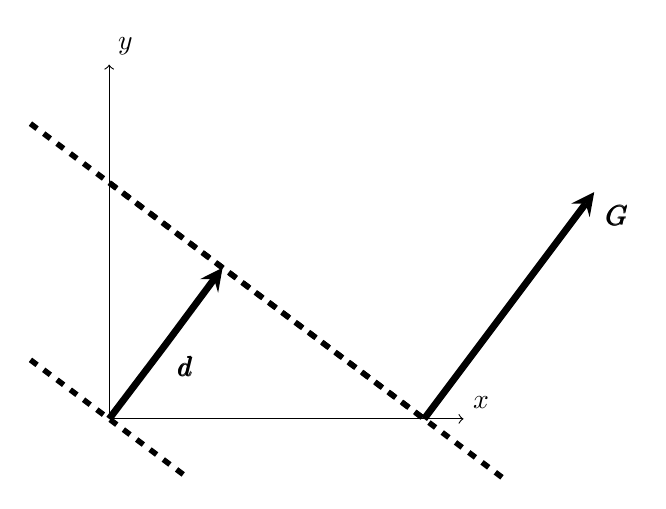
\begin{tikzpicture}
    \draw[->] (0, 0) -- (4.5, 0) node[anchor = south west] {$x$};
    \draw[->] (0, 0) -- (0, 4.5) node[anchor = south west] {$y$};
    \draw[dashed, line width = 2] (-1, 3.75) -- (5, -0.75);
    \draw[dashed, line width = 2] (-1, .75) -- (1, -0.75);
    \draw[dashed, line width = 2] (0, 3) -- (4, 0);
    \draw[->, line width = 2.5, >=stealth] (0, 0) --  (0.72, 0.95) node[anchor = north west] {$\pmb{d}$}-- (1.44, 1.92);
    \draw[->, line width = 2.5, >=stealth] (4, 0) -- (6.16, 2.88) node[anchor = north west] {$\pmb{G}$};
  \end{tikzpicture}
  \caption{The interplanar separation.}
  \label{fig:planeSep}
\end{figure}

\begin{figure}
  \centering
  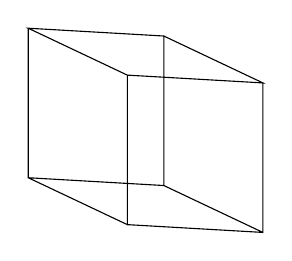
\begin{tikzpicture}
    \begin{axis}[
      axis x line=none,
      axis y line=none,
      axis z line=none,
      axis equal image,
%      view = {20}{30}
    ]
    \addplot3 [mark=none] coordinates 
    {
      (0, -1, 2)
      (3, 0, 2)
      (0, 1, 2)
      (-3, 0, 2)
      (0, -1, 2)
      (0, -1, -2)
      (3, 0, -2)
      (3, 0, 2)
      (3, 0, -2)
      (0, 1, -2)
      (0, 1, 2)
      (0, 1, -2)
      (-3, 0, -2)
      (-3, 0, 2)
      (-3, 0, -2)
      (0, -1, -2)
      (0, -1, 2)
      (0, -1, -2)
    };
    \end{axis}
  \end{tikzpicture}
  \caption{The first Brillouin zone of a hexagonal lattice}
  \label{fig:firsBrillouin}
\end{figure}

2.
\begin{minipage}[t]{0.9\textwidth}
  a).
  \begin{minipage}[t]{\textwidth}
    The volume of the primitive cell is given by:
    \begin{equation*}
      V = \af \dprod (\as \times \at)
    \end{equation*}
    We have:
    \begin{equation*}
      \as \times \at = - \sqrt{3}\frac{ac}{2} (- \uv{y}) + \frac{ac}{2} \uv{x} = \sqrt{3}\frac{ac}{2} \uv{y} + \frac{ac}{2} \uv{x}
    \end{equation*}
    Thus:
    \begin{equation*}
      V = \frac{\sqrt{3} a^2c}{4} + \frac{\sqrt{3} a^2c}{4} = \sqrt{3} \frac{a^2c}{2}
    \end{equation*}\\
  \end{minipage}
  b).
  \begin{minipage}[t]{\textwidth}
    We have by the definition of the reciprocal lattice vectors:
    \begin{equation*}
      \uv{b_1} = 2 \pi \frac{\as \times \at}{V} = \frac{2 \pi}{V}
      \left|
      \begin{matrix}
        \uv{x} & \uv{y} & \uv{z}\\
        -\frac{\sqrt{3}a}{2} & \frac{a}{2} & 0\\
        0 & 0 & c
      \end{matrix}
      \right|
      = \frac{2 \pi}{\sqrt{3}ac} \uv{x} + \frac{2\pi}{a}\uv{y}
    \end{equation*}
    \begin{equation*}
      \uv{b_2} = 2 \pi \frac{\at \times \af}{V} = \frac{2 \pi}{V}
      \left|
      \begin{matrix}
        \uv{x} & \uv{y} & \uv{z}\\
        0 & 0 & c\\
        \frac{\sqrt{3}a}{2} & \frac{a}{2} & 0
      \end{matrix}
      \right|
      =  - \frac{2 \pi}{\sqrt{3}ac} \uv{x} + \frac{2\pi}{a}\uv{y}
    \end{equation*}
    \begin{equation*}
      \uv{b_3} = 2 \pi \frac{\af \times \as}{V} = \frac{2 \pi}{V}
      \left|
      \begin{matrix}
        \uv{x} & \uv{y} & \uv{z}\\
         \frac{\sqrt{3}a}{2} & \frac{a}{2} & 0\\
        -\frac{\sqrt{3}a}{2} & \frac{a}{2} & 0
      \end{matrix}
      \right|
      = \frac{2 \pi}{V}\frac{\sqrt{3}a^2 - (-\sqrt{3}a^2)}{2}
      = \frac{2 \pi}{c} \uv{z}
    \end{equation*}
  \end{minipage}

  c).
  \begin{minipage}[t]{\textwidth}
    The first Brillouin zone is described by the planes that bisect the following vectors perpendicularly:
    \begin{gather*}
      \frac{2 \pi}{\sqrt{3}ac} \uv{x} + \frac{2\pi}{a}\uv{y}\\
      - \frac{2 \pi}{\sqrt{3}ac} \uv{x} - \frac{2\pi}{a}\uv{y}\\
      -\frac{2 \pi}{\sqrt{3}ac} \uv{x} + \frac{2\pi}{a}\uv{y}\\
      \frac{2 \pi}{\sqrt{3}ac} \uv{x} - \frac{2\pi}{a}\uv{y}\\
      \pm \frac{2 \pi}{c} \uv{z}\\
    \end{gather*}
    This can be seen in Fig.~\ref{fig:firsBrillouin},
    it is a rhombic prism.
  \end{minipage}
\end{minipage}
\end{document}
